%!TEX root = ../../super_main.tex

\section{The Campaign Model}

Conceptually, a \emph{snapshots} is a snippet of the reality (context) that a specific participants exists in, measured through the subjects devices along with a \emph{label}, describing this reality further. This label is used to define the reality in ways that available sensors cannot. 

% Vi kigger på snapshots, og deres label. Vi kan nu se mønstre i målingerne, og tilføje mere viden til de målinger. Eksempelvis kunne man undersøge om der var en sammenhæng mellem en alternated puls, og dét at være fuld.

By examining snapshots, and their labels, customers will be able to recognize patterns in measurements, and be able to see a correlation between sensor output and human dynamics. However, to allow customers to gather data that they want in the first place we want to enable them to specify how, what and when snapshots should be gathered. For this reason we have the concept of a \emph{campaign}, which is a recipe for the snapshots the customer desires. A \emph{campaign} is a specification of what type of sensor data, the timings and frequencies of the measurements and a way of deriving the \emph{label} from the participants.

% BAJER EKESEMPEL
For instance if a customer want to investigate how the consumption of alcohol affects the reality of the participants, they might specify a \emph{campaign} where they want to gather data from a hear rate sensor, an accelerometer, and a GPS location. They will further have to specify how often they want to eaves drop on these sensors alongside a questionnaire with questions that can help them learn how alcohol and these sensor output correlates. An example of a snapshot corresponding to such a \emph{campagin} can be seen in \figref{fig:snapshot_example}.

The reality of the participants are measured through a series of \emph{samples}, each consisting of a sequence of \emph{measurements}.
\\\\
\figref{fig:snapshot_example} shows an example of a snapshot where three sensors are used. The measurements from these sensors are then labeled, further describing the context of the participants. In this example, participants are asked to rate how drunk they are. This information can then, later, be used to 

\begin{figure}[!htbp]
    \centering
    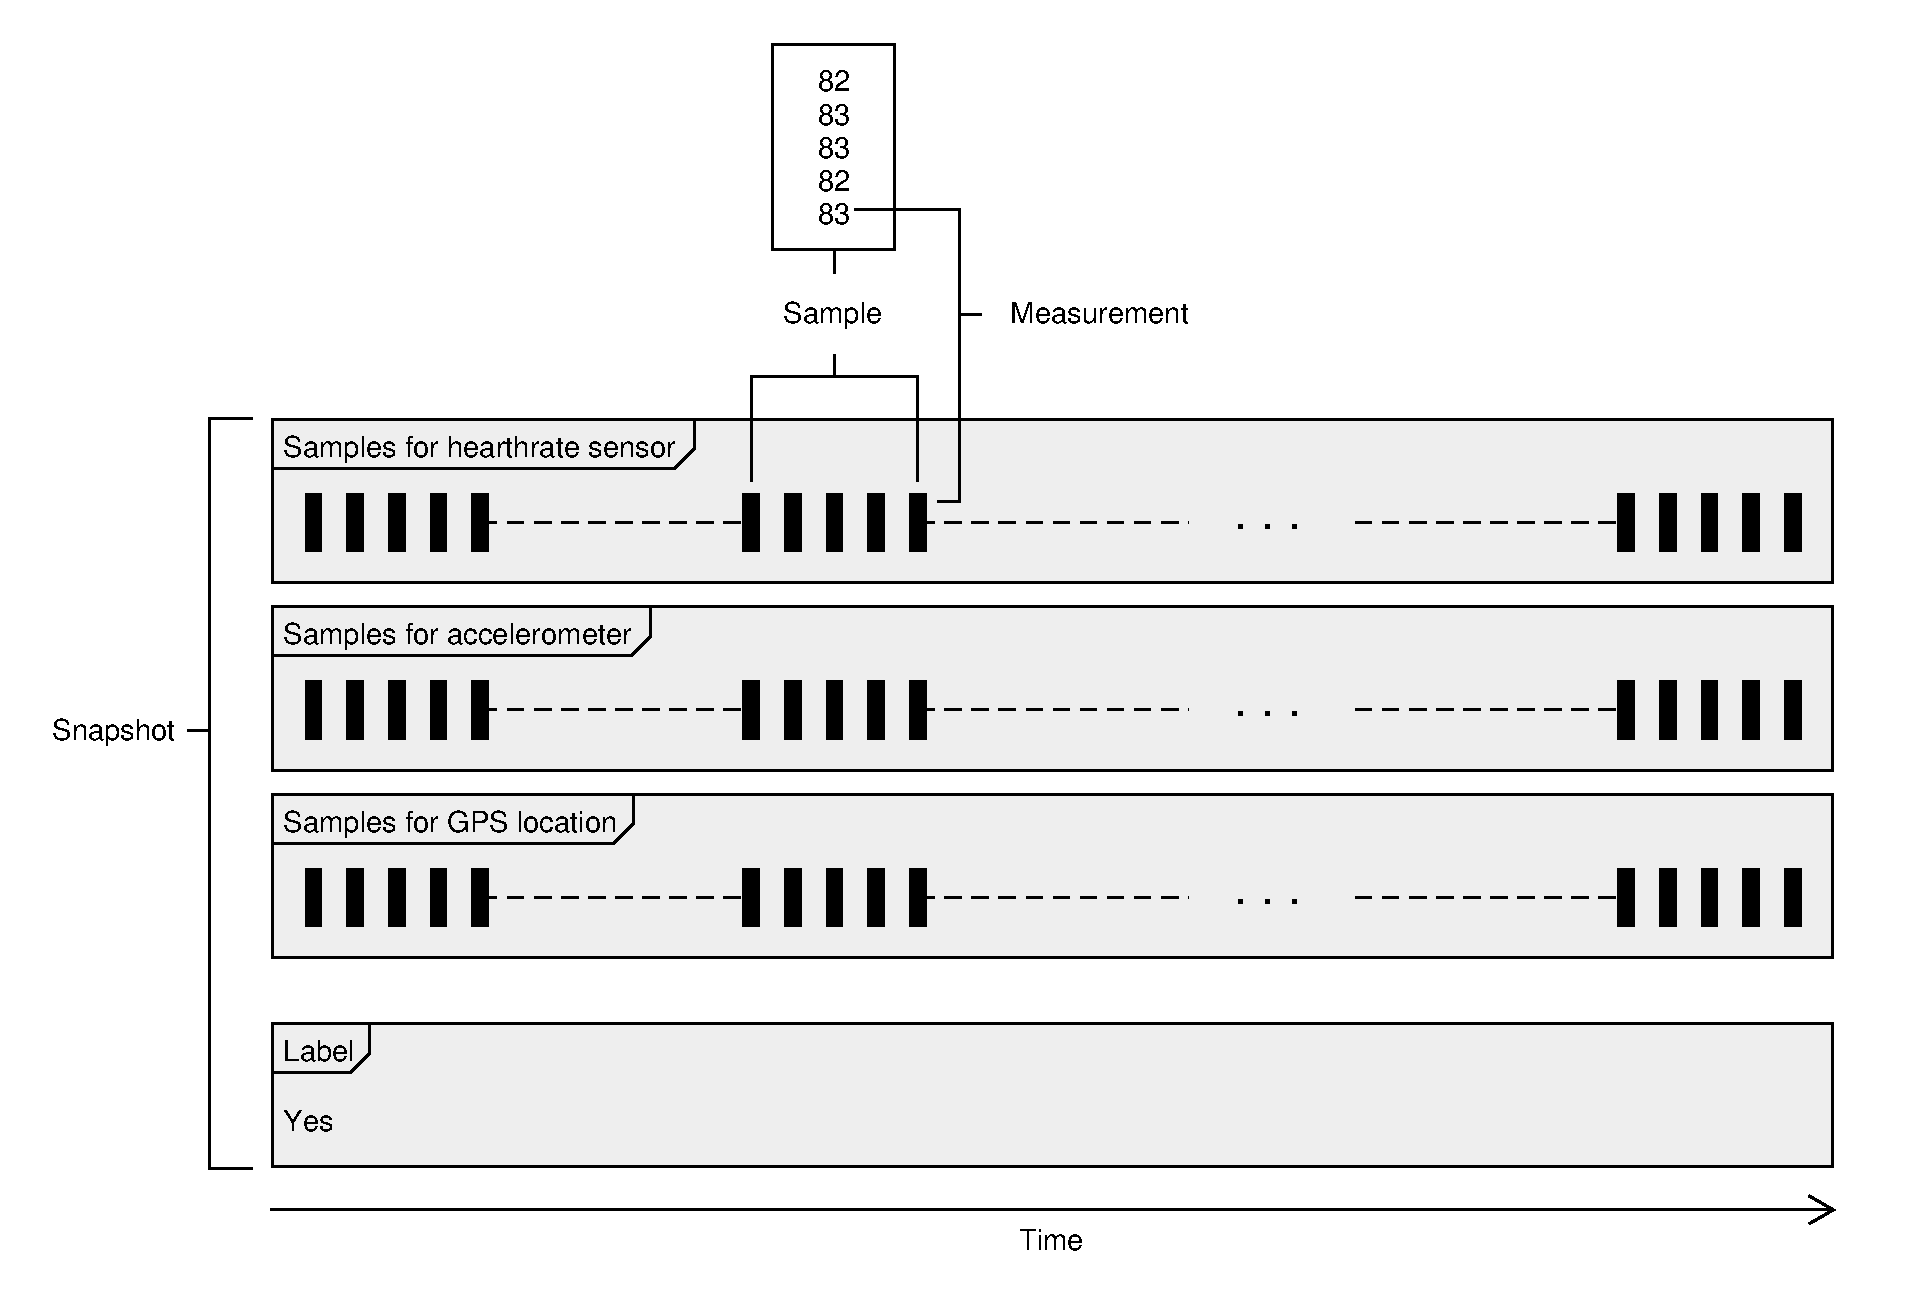
\includegraphics[width=\textwidth]{gathering_sensor_data/snapshot}
    \caption{Snapshot.}
    \label{fig:snapshot_example}
\end{figure}
\FloatBarrier

An example of such a snapshot could be as seen in \figref{fig:snapshot_example}. This have outputs from the sensors specified in the campaign. These measurements have some special temporal structure which will be described REF-TIL-TEMPORALITY. Besides sensor readings a \emph{snapshot} also have a \emph{label} associated. 

\todo[inline]{Beskriv hvad en campaign er i koden, brug gerne klassediagrammet til at forklare det!}

\begin{figure}[!htbp]
    \centering
    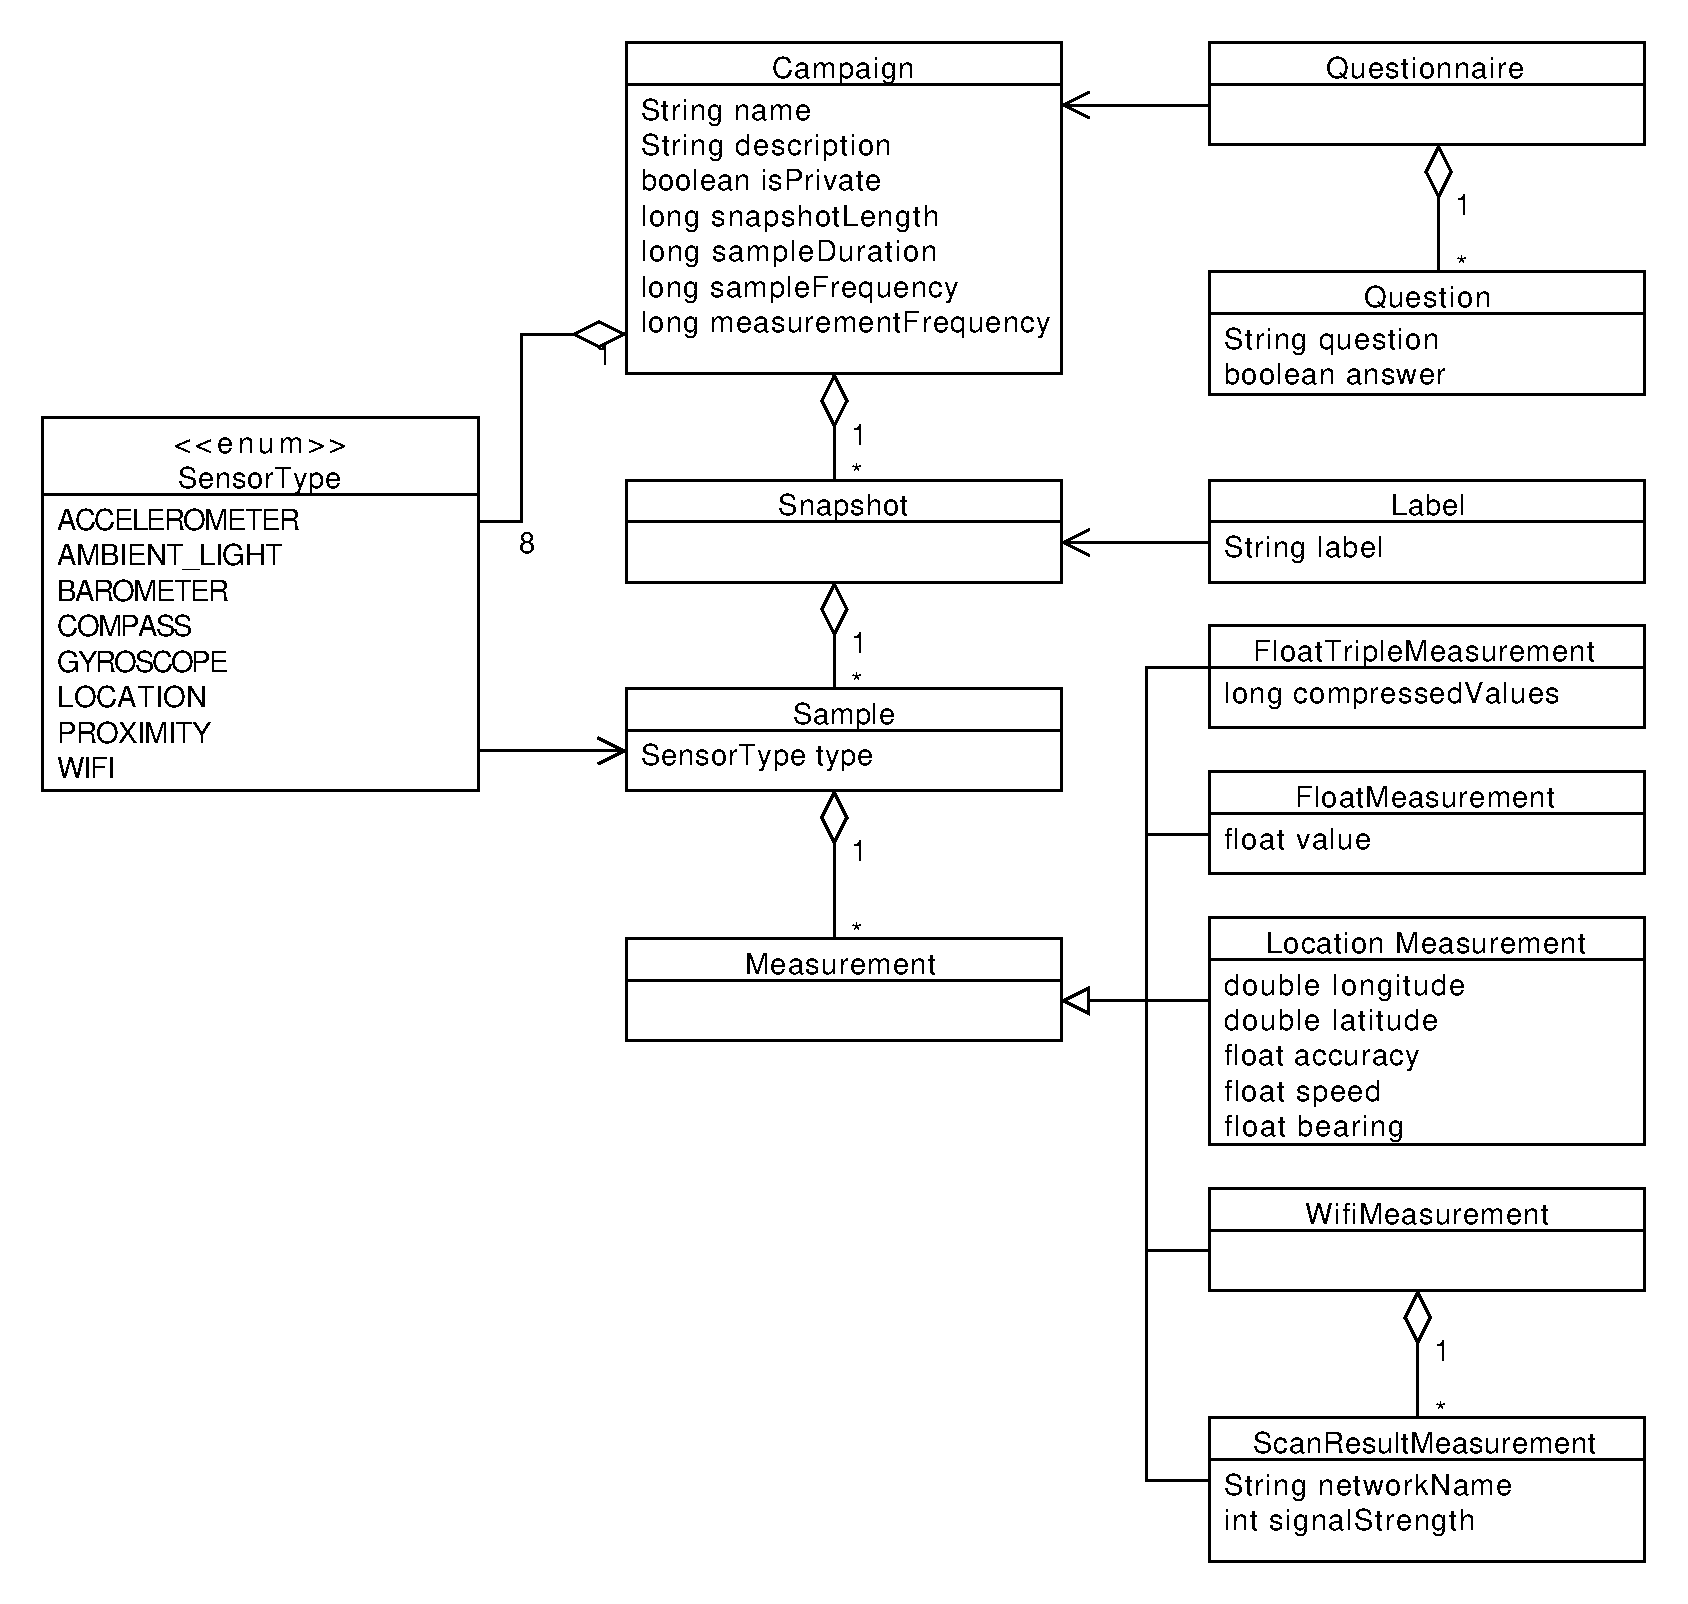
\includegraphics[width=\textwidth]{graphic/gathering_sensor_data/model_class_diagram.pdf}
    \caption{Class Diagram of the campaign model.}
    \label{fig:model_class_diagram}
\end{figure}
\FloatBarrier

\todo[inline]{ref til figur}

\subsection{Questionnaires}
We had come to the conclusion that customers should be able to define questionnaires to be a part of the data collection \secref{sec:human_activity_recognition}. Customers should be able to define one or more separate questions or more generally data inputs which combined should make out a questionnaire model. 
\\\\
Simple boolean yes/no questions can directly be combined to create a discrete amount of labels or classes which can later be used as targets for an AI model but more open inputs, which for instance can be used for regression or as more diverse features, should also be possible. \todo{Overvej om vi når at implementere continuous inputs}
\\\\
A questionnaire specification should be transformable to a format which can be easily be parsed and send from the server to the collecting devices. We have therefore implemented a questionnaire to be Java Parcelable. \todo{Overvej at ændre det her hvis vi gør det til JSON ting i stedet}

